\documentclass{ali-poster}

\usepackage{graphicx}
\usepackage{qrcode}
\usepackage{ali-macros, ali-pseudocode, ali-crypto}

% diagram preamble material
\usepackage{tikz}
\usepackage{tikzpeople}
\usepackage{fontawesome}
\usetikzlibrary{positioning}
\usetikzlibrary{shapes.callouts}

\definecolor{packergreen}{RGB}{24,80,40}
\definecolor{packeryellow}{RGB}{255,184,28}
\definecolor{vikingpurple}{RGB}{79,38,131}
\definecolor{vikingyellow}{RGB}{255,198,47}


\title{Balancing Privacy and Accountability on Encrypted  Messaging Platforms}
\author{Alistair Pattison and Nicholas Hopper}
\date{S\&P Oakland, May 2023}

\begin{document}
% 
% ------------------
% -- LEFT PANEL -- 
% ------------------
% 
\noindent%
\begin{panel}{\sidebarwidth}{sidebarcolor}

	\section*{The Protocol}

	This work extends a protocol by Issa, Alhaddad, and Varia called Hecate. In the Hecate protocol, every message sent via an encrypted service requires a token containing (among other things), the encryption
	\begin{equation*}
		x_1 \ceq \Enc_{mod}(id_{src}).
	\end{equation*}
	This $x_1$ is attached to a sent message so that if the message is reported, a moderator can decrypt $x_1$ to recover the sender's identity.
	Using threshold cryptography, this work extends Hecate so that the source's identity is revealed only under sufficient agreement from a group of moderators.

	\vspace{1cm}

	% -- PSEUDOCODE -- 
	\begin{algorithmic}[1]
		\function{CreateToken}{$id_{usr}$}{
			\State Compute $x_1 = \Enc(id_{src})$ using a $k$ out of $n$ threshold encryption scheme.
			\State Package $x_1$ into a token and send a signature request to each moderator.
			\State Each moderator verifies verifies $x_1$ and returns their signature share on the token.
			\State Once sufficient responses are received, combine the shares into into a valid signature.
		}
	\end{algorithmic}

	\vspace{1cm}

	\begin{algorithmic}[1]
		\function{HandleReport}{$m$, $x_1$}{
			\State A user sends a request to all $n$ moderators containing the reported message $m$ and the encrypted id, $x_1 = \tuple{c_1, c_2}$.
			\State If a moderator believes that the message is worth acting upon, she forwards the decryption share $d_i$ to the appropriate authorities.
			\State If enough decryption shares are received, one combines the decryption shares to recover $x_1$.
		}
	\end{algorithmic}

	\medskip

	\section*{Implementation}

	We implement the protocol using Rust and run each party in a separate container communicating over HTTP. We estimate the cost of adoption to be around around \$100 per day for the entirety of WhatsApp. See the poster abstract for benchmark results.

\end{panel}%
\hspace{\marginwidth}
% 
% ------------------
% -- CENTER PANEL -- 
% ------------------
% 
\begin{panel}{\centerwidth}{white}
	% -- TITLE -- 
	\maketitle

	\vspace{2cm}

	% -- SHORT SUMMARY -- 
	\hfill\parbox{\dimexpr\centerwidth-4cm\relax}{
		\LARGE
		This work introduces a protocol in which {\bf\color{highlightcolor1} the sender of an abusive message can be verified if there is sufficient agreement among a group of moderators}.
		The protocol {\bf\color{highlightcolor2} retains all security properties of the messaging service for unreported messages}.

	}\hfill\null

	\vspace{4cm}

	\begin{center}
		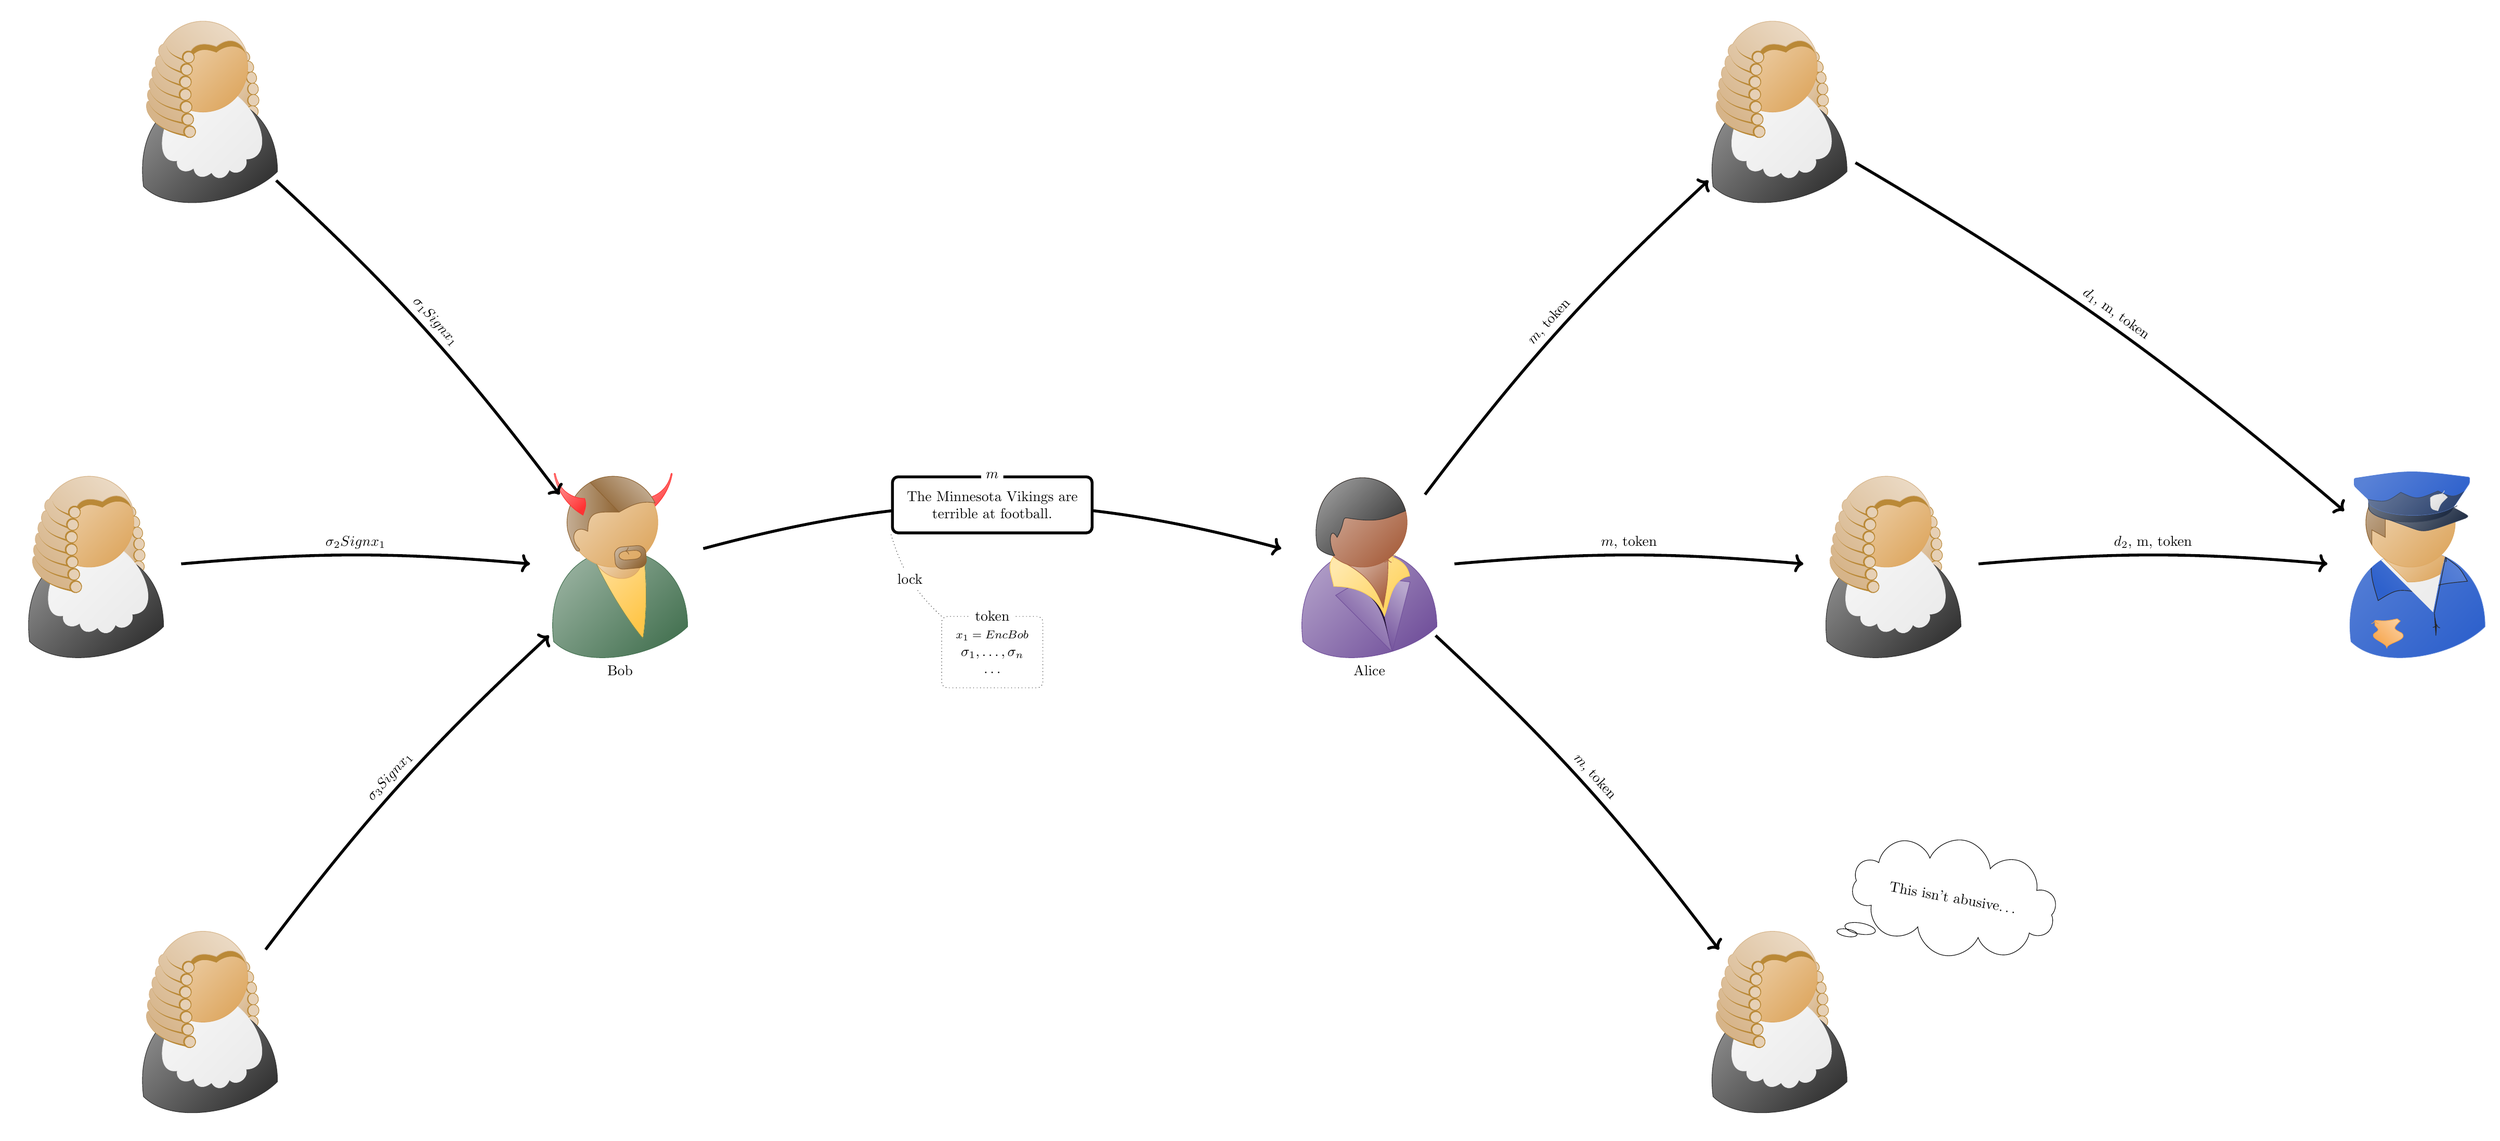
\begin{tikzpicture}
	[
		node distance = 9.5cm,
		->,
	]

	% draw all the characters
	\begin{scope}[
			nodes = {minimum width = 3.3cm}
		]
		% sender
		\node [
			bob,
			evil,
			shirt = packergreen,
			undershirt = packeryellow
		] (bob) {Bob};

		% recipient
		\node [
			alice,
			right = 15cm of bob,
			shirt = vikingpurple,
			undershirt = vikingyellow,
		] (alice) {Alice};

		% signing mods
		\node [judge, above left = of bob] (signer-1) {};
		\node [judge, left = of bob] (signer-2) {};
		\node [judge, below left = of bob] (signer-3) {};

		% judging mods
		\node [judge, female, above right = of alice] (judge-1) {};
		\node [judge, right = of alice] (judge-2) {};
		\node [judge, below right = of alice] (judge-3) {};

		% police
		\node [police, right = of judge-2] (police) {};

	\end{scope}

	% the message itself
	\begin{scope}[
			bend angle = 15,
			bend left,
			nodes = {
					rounded corners,
					align = center,
					fill = white
				}
		]

		% abusive message
		\draw [line width = 2pt] {
			(bob) to
			node [inner sep = 1em, draw] (message) {
					The Minnesota Vikings are \\
					terrible at football.}
			(alice)
		};

		% message label
		\node at (message.north) [fill = white] {$m$};

		% token
		\node [
			below = 2cm of message,
			draw, dotted,
			inner sep = 1em
		] (token) {
			\footnotesize
			$x_1 = \Call{Enc}{\text{Bob}}$ \\
			$\sigma_1, \ldots, \sigma_n$ \\
			$\dots$
		};

		\draw[-., dotted] (token.north west) to node {\faicon{lock}} (message.south west);

		% token label
		\node at (token.north) [fill = white] {token};
	\end{scope}

	% --- MODERATOR INTERACTION ---
	\begin{scope}[
			bend angle = 5,
			bend left,
			nodes = {sloped, above},
			line width = 2pt
		]
		% getting moderator signatures
		\foreach \i in {1, 2, 3}
		\draw {
			(signer-\i) to
			node {$\sigma_\i \ceq \Call{Sign}{x_1}$}
			(bob)
		};

		% requesting decryption shares
		\foreach \i in {1, 2, 3}
		\draw {
			(alice) to
			node {$m$, token}
			(judge-\i)
		};

		% responses
		\foreach \i in {1, 2}
		\draw {
			(judge-\i) to
			node {$d_\i$, m, token}
			(police)
		};
	\end{scope}

	% --- THOUGHT BUBBLES ---
	\begin{scope}[
			nodes = {
					cloud callout,
					draw,
					aspect = 2.7,
					fill = white
				}
		]

		% decryption
		% \node [
		% 	node distance = .5em and 1em,
		% 	above right = of police,
		% 	callout absolute pointer={(police.north east)},
		% ] {
		% 	$\text{Bob} = \Call{Dec}{x_1, (d_1, d_2)}$
		% };

		% dissenting moderator 
		\node[
			node distance = .5em and 2em,
			above right = of judge-3,
			callout absolute pointer={(judge-3.north east)},
			rotate = -10,
		] {This isn't abusive\dots};
	\end{scope}

	% --- DECRYPTION ---

\end{tikzpicture}

	\end{center}

	% -- NEWSPAPER HEADLINES --
	% \begin{center}
	% 	\scalebox{.75}{\parbox{\centerwidth}{
	% 			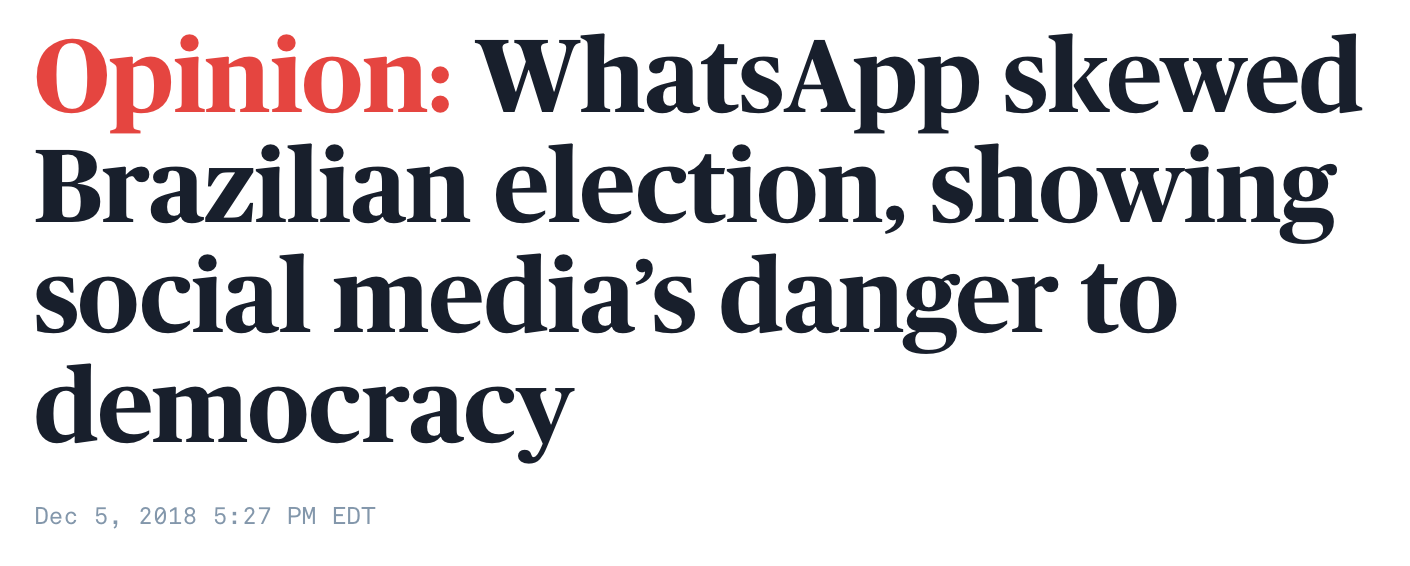
\includegraphics{graphics/brazil-election.png}
	% 			\hspace{2cm}
	% 			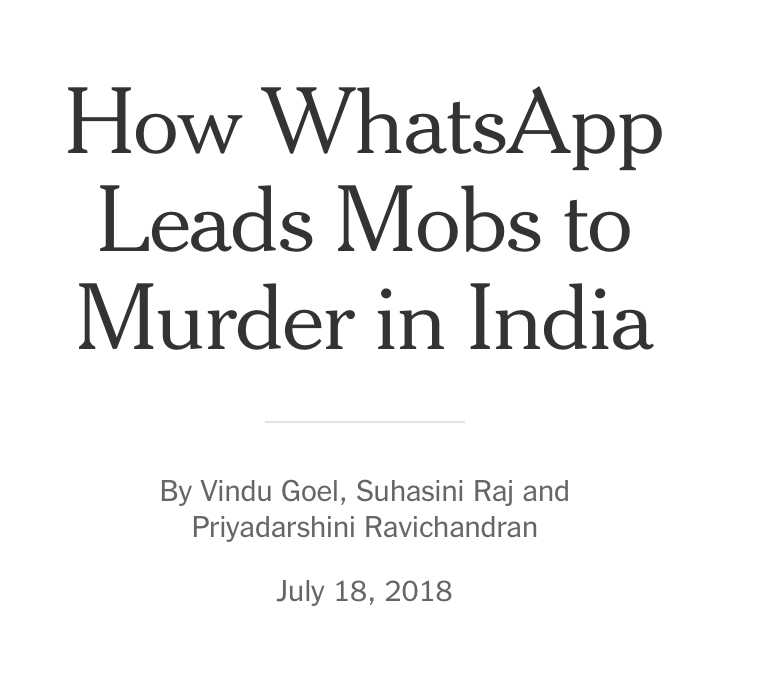
\includegraphics{graphics/india-murder.png}

	% 			\hfill 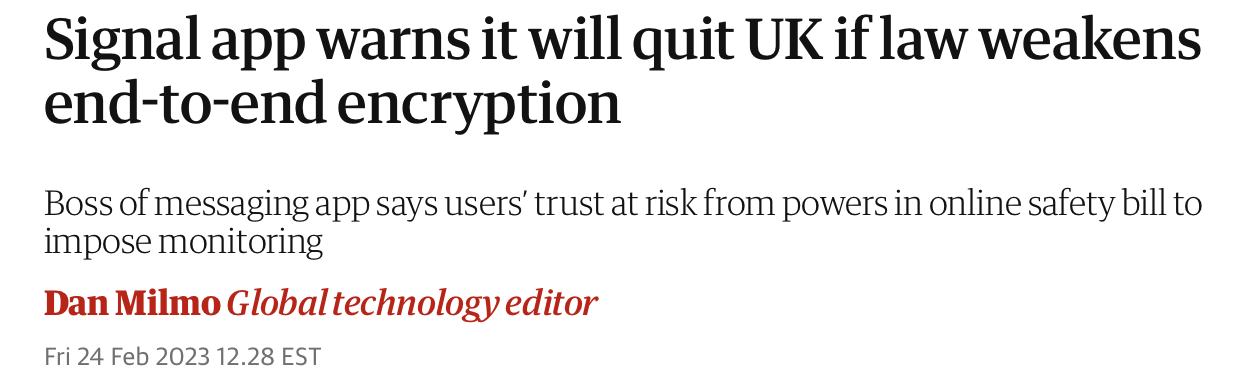
\includegraphics[scale=1.25]{graphics/signal-uk.png} \hfill\null
	% 			\bigskip\bigskip

	% 			\hspace{3cm}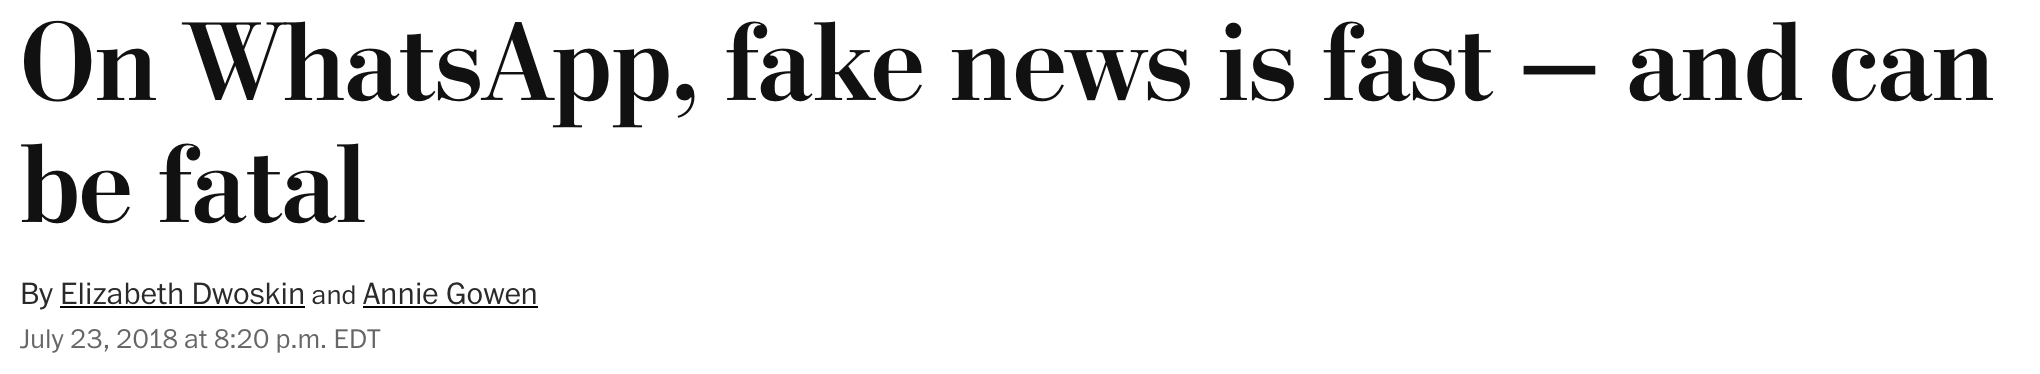
\includegraphics{graphics/fake-news.png}
	% 		}}
	% \end{center}

\end{panel}%
\hspace{\marginwidth}
% 
% -------------------
% -- RIGHT PANEL --
% -------------------
% 

\qrset{
	height=.4\footerheight,
	version=6,
}
\footer{
	\parbox[c][\footerheight]{.5\textwidth}{%
		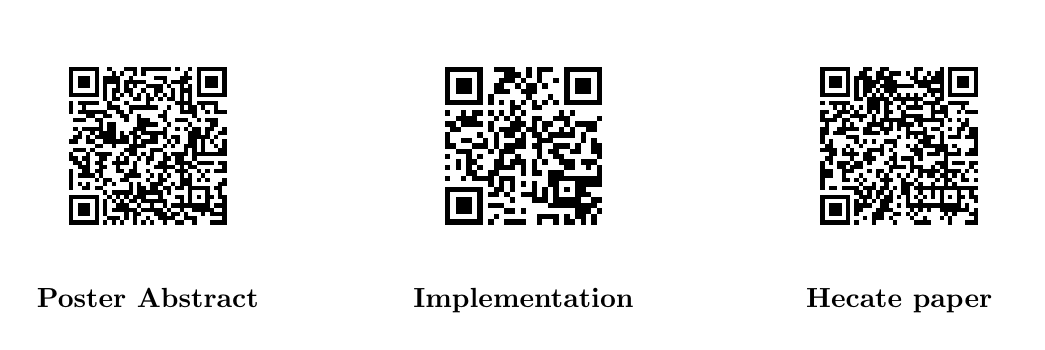
\begin{tikzpicture}[
				node distance = .5em and 5em,
				font = \bfseries,
				align = center,
				qr/.style = {
						font = \color{black},
						fill = white,
						inner sep = 5mm,
						rounded corners = 3mm
					}
			]

			% poster abstract
			\node[qr] (abstract) {\qrcode{%
					https://raw.githubusercontent.com/alipatti/cerberus/master/writeup/main.pdf}};
			\node[below = of abstract] {Poster Abstract};

			% implementation
			\node[qr, right = of abstract] (github) {\qrcode{%
					http://github.com/alipatti/cerberus}};
			\node[below = of github] {Implementation};

			% original hecate paper
			\node[qr, right = of github] (hecate) {\qrcode{%
					https://www.usenix.org/conference/usenixsecurity22/presentation/issa}};
			\node[below = of hecate] {Hecate paper};
		\end{tikzpicture}
	}
	\parbox[c][\footerheight]{.5\textwidth}{%
		\hfill
		\begin{tikzpicture}[
				node distance = 1em,
			]
			\node (nsf) {
				
\includegraphics[height=.5\footerheight]{logos/nsf-logo.png}};
			\node [right = of nsf] (umn) {
				
\includegraphics[height=.4\footerheight]{logos/umn-logo.png}};
			\node [right = of umn] (carleton) {
				
\includegraphics[height=.5\footerheight]{logos/carleton-logo.png}};
		\end{tikzpicture}
	}
}

\end{document}